\subsection{Высокоуровневый обзор}
Высокоуровневое архитектурное представление cистемы сфокусировано на взаимодействии с пользователями и потоке данных, связанных с данными, отправляемыми пользователями.

\textbf{Управление пользователями:}
\noindent
\begin{itemize}
    \itemsep 0em
    \item Пользователи регистрируются в системе, предоставляя основную информацию, такую как имя пользователя и электронная почта. Дополнительные сведения о профиле, такие как имя, местоположение и принадлежность, фиксируются в отдельной таблице.
   \item Система сможет различать роли пользователей с помощью флагов (is\_staff), что позволяет использовать механизмы гранулярного контроля доступа.
\end{itemize}

\textbf{Обработка решений:}
\noindent
\begin{itemize}
    \itemsep 0em
    \item Пользователи отправляют данные по установленным каналам, и система записывает ссылку на исходный код и временную метку отправки для каждого экземпляра.
    \item Центральная система очередей, работающая на базе Celery, эффективно управляет обработкой поступающих решений, обеспечивая оптимальное использование ресурсов.
    \item Предоставленные данные надежно хранятся в облачном хранилище, используя его масштабируемость и гибкость для работы с различными форматами данных.
\end{itemize}

\textbf{Сохранение данных:}
\noindent
\begin{itemize}
\itemsep 0em
    \item Данные о пользователях, включая информацию о профиле и историю активности, хранятся в базе данных MySQL. Эта реляционная структура базы данных позволяет эффективно выполнять запросы и управлять структурированными данными.
    \item Данные об отправке решений хранятся в базе данных MongoDB, что позволяет использовать ее масштабируемость и гибкость при работе с потенциально большими и неоднородными форматами данных.
\end{itemize}

% \subsection{Балансировка нагрузки}

% \subsection{Мониторинг}

\subsection{Обзор пути обработки решений}
% \begin{figure}[p]
%     \centering
%     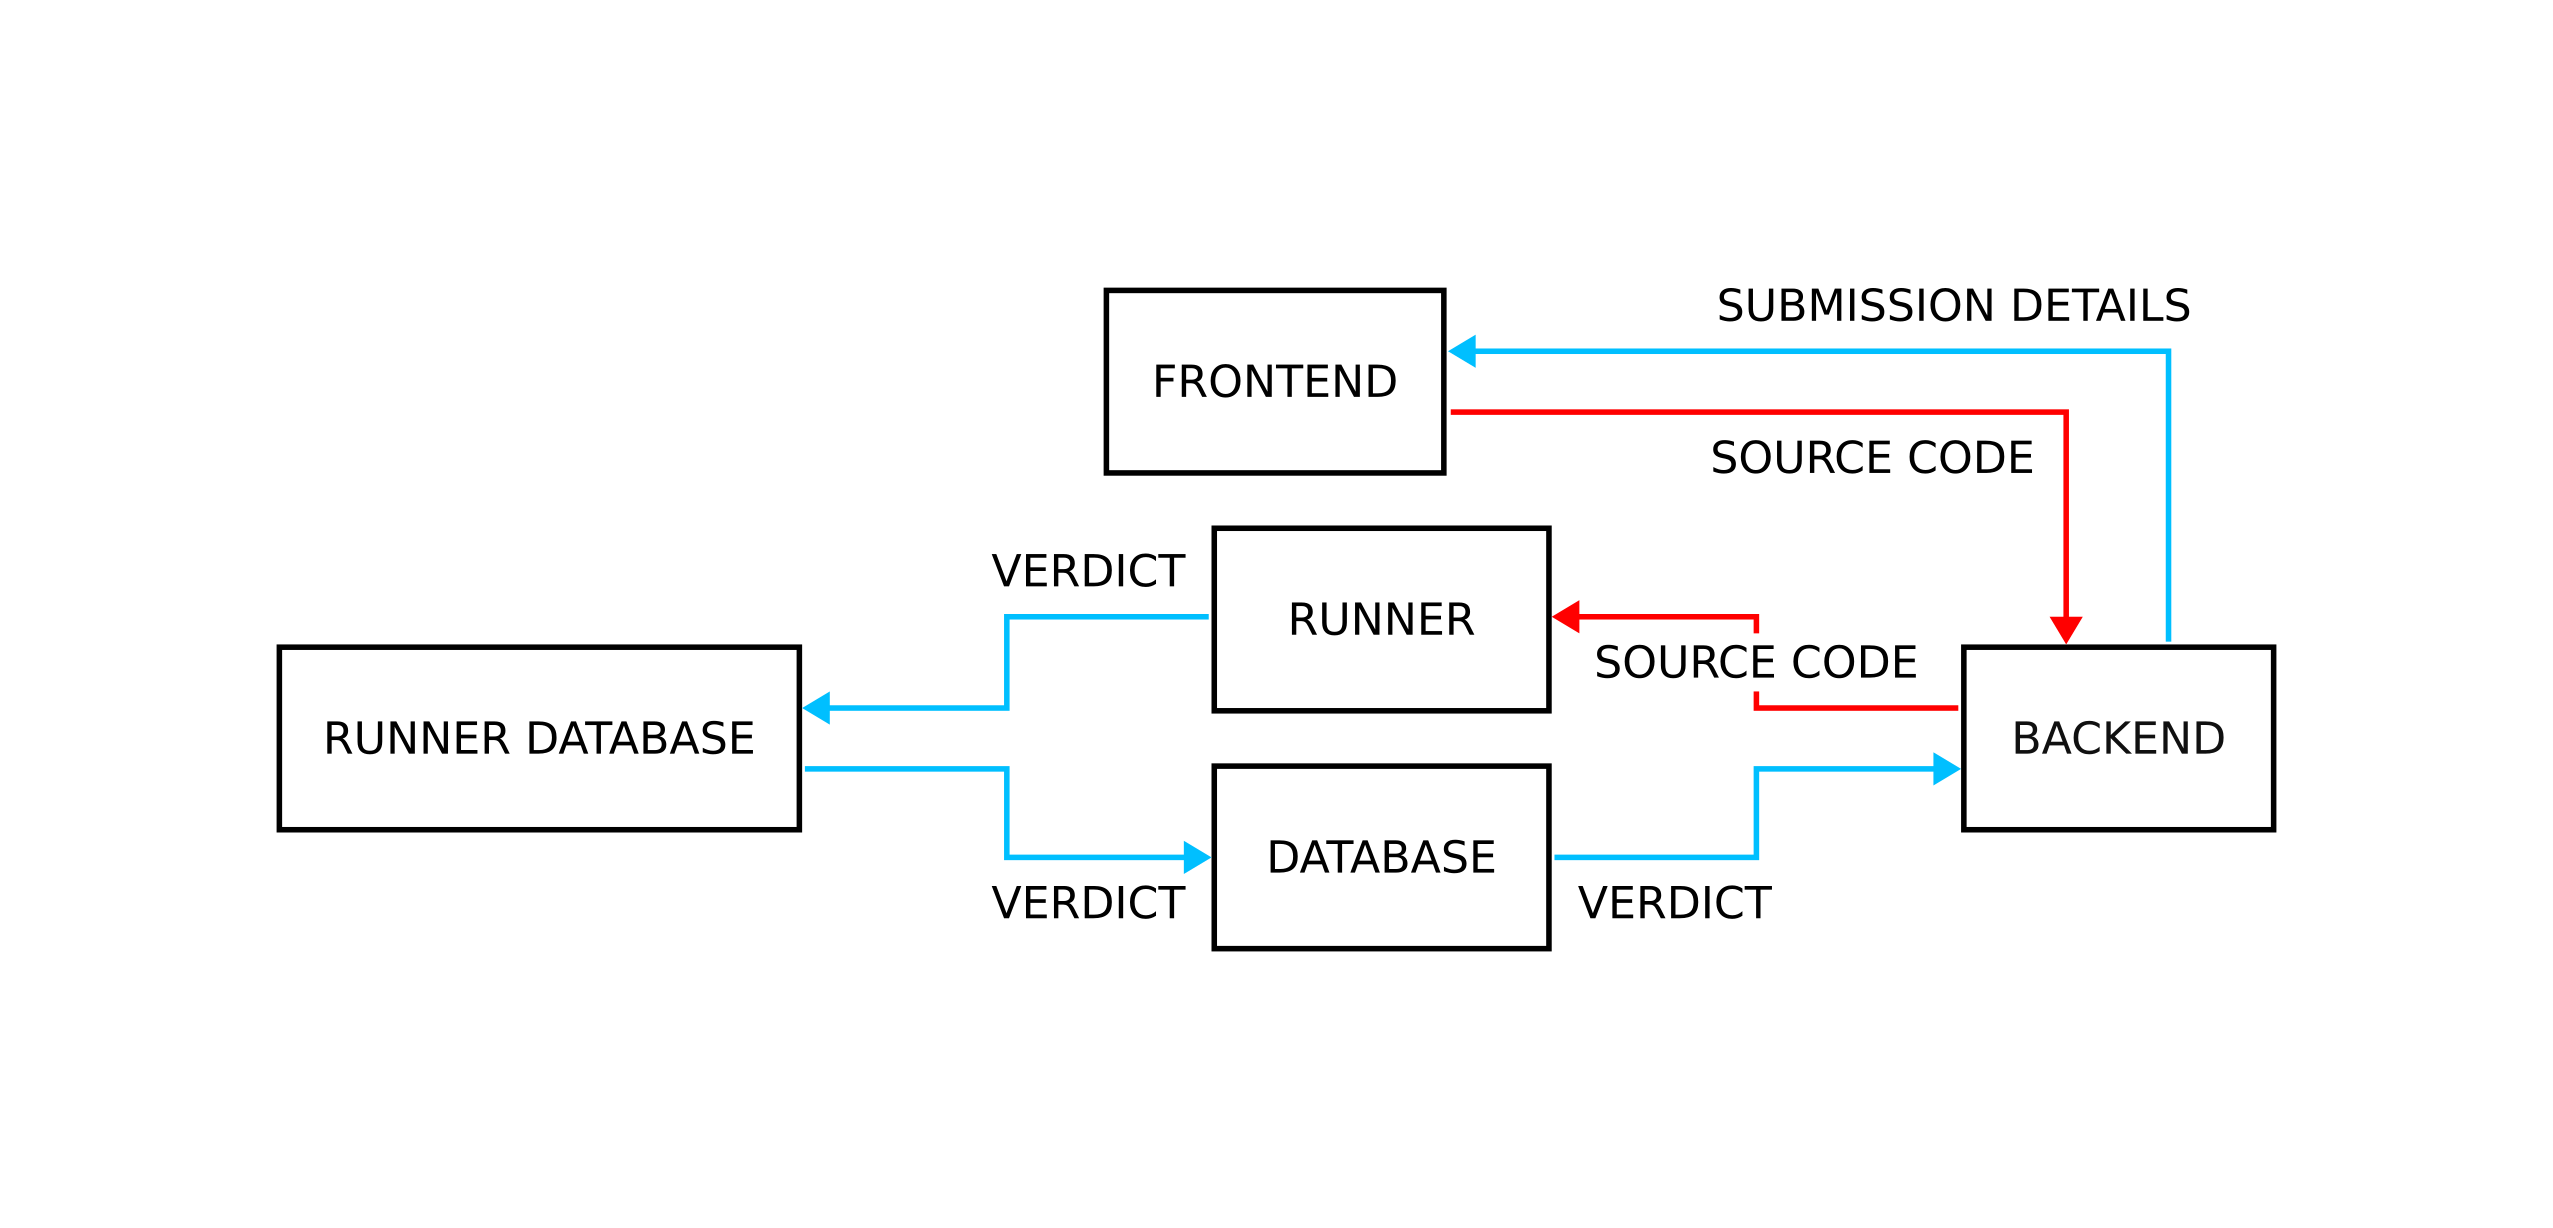
\includegraphics[width=0.8\textwidth]{submission_process.png}
%     \caption{Путь обработки решения}
% \end{figure}


\subsubsection{Выбор контайнера и распределенное выполнение}
\begin{figure}[h]
    \centering
    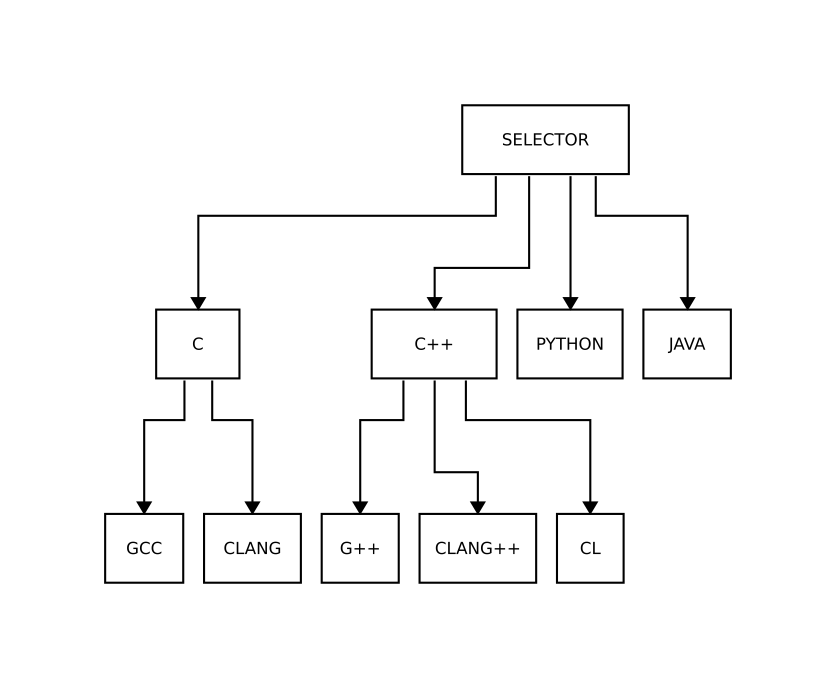
\includegraphics[width=0.8\textwidth]{selector.png}
    \caption{Схема выбора контайнера исполнения}
    \noindent
\end{figure}

\noindent

Перед выполнением Veritas применяет стратегии тщательного выбора контейнеров (в первой версии производится силами пользователя):
\begin{itemize}
    \itemsep 0em
    \item \textbf{Подбор языка и фреймворка:} система использует специальный реестр контейнеров, в котором хранятся готовые образы для популярных языков программирования и фреймворков. На основе идентификации языка и фреймворка представленного кода из реестра выбирается наиболее подходящий контейнер.
    \item \textbf{Управление версиями:} Veritas поддерживает несколько версий контейнеров для каждого языка/фреймворка, что позволяет организаторам определять желаемую среду выполнения для конкретных соревнований или упражнений. Такая гибкость позволяет удовлетворить различные требования и предпочтения.
    \item \textbf{Соображения безопасности:} Механизмы "песочницы" в контейнерах дополнительно повышают безопасность, ограничивая доступ к файловой системе и сетевое взаимодействие.
\end{itemize}

\subsubsection{Выполнение тестов и возврат вердиктов}
После выбора оптимального контейнера начинается фаза выполнения:
\begin{itemize}
    \itemsep 0em
    \item \textbf{Подготовка контейнера:} Эфемерный экземпляр контейнера запускается с использованием выбранного образа. В среду контейнера вводятся необходимые параметры конфигурации и данные тестовых примеров.
    \item \textbf{Изолированное выполнение:} Представленный код выполняется в контейнере, полностью изолированном от базовой хост-системы. Это гарантирует справедливость и устраняет проблемы совместимости, связанные с различными программными средами.
    \item \textbf{Управление ресурсами:} Система использует методы управления ресурсами для обеспечения эффективного распределения вычислительных ресурсов между запущенными контейнерами. Это позволяет оптимизировать производительность системы и предотвратить нехватку ресурсов, особенно в периоды пиковых нагрузок.
    \item \textbf{Мониторинг выполнения:} \textit{(Отложено до v2)} На протяжении всего этапа выполнения система отслеживает использование ресурсов и состояние контейнеров. Любые аномалии или истощение ресурсов вызывают корректирующие действия, обеспечивая плавное и бесперебойное выполнение.
\end{itemize}


\subsubsection{Агрегация и хранение вердиктов}
\begin{figure}[h]
    \centering
    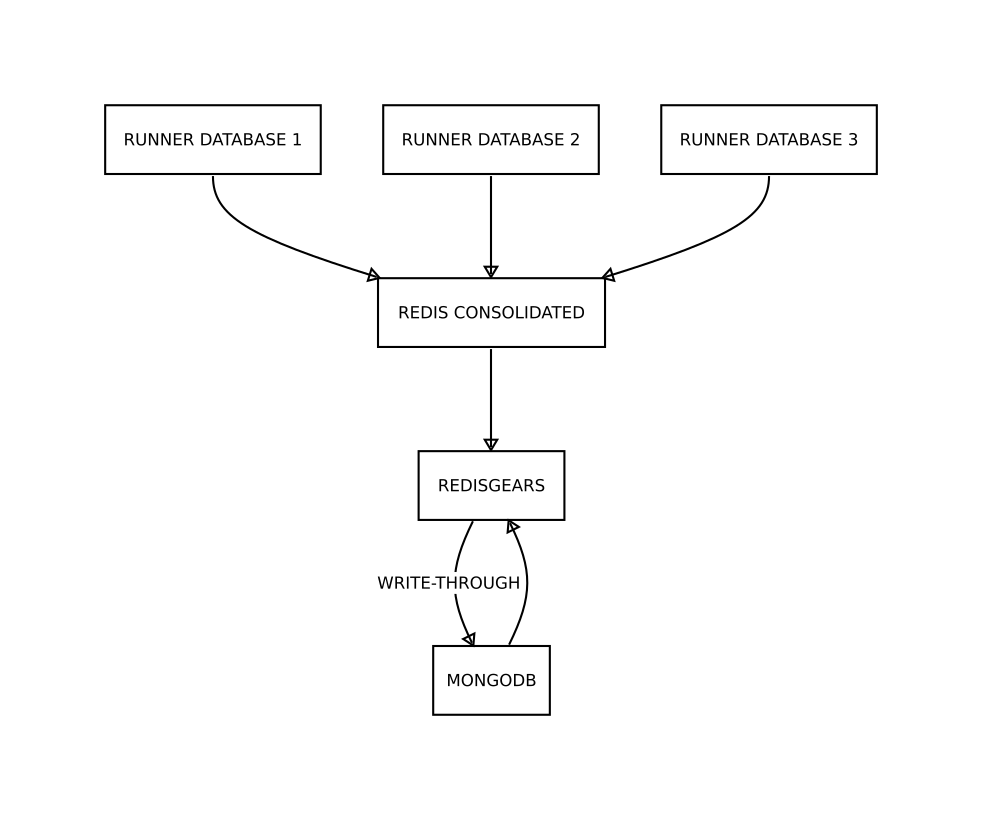
\includegraphics[width=0.8\textwidth]{aggregation.png}
    \caption{Схема агрегации вердиктов}
    \noindent
\end{figure}
Поскольку представления выполняются в изолированных контейнерах, формирование вердиктов приобретает первостепенное значение.

\textbf{Распределенная генерация вердиктов:}
\noindent
Каждый прогонщик, выполнив представленный образец кода с тестовыми примерами, генерирует вердикт. Этот вердикт содержит результат (пройден, не пройден, ошибка), а также другие важные данные, такие как время выполнения и использование ресурсов.
Система использует метод pub/sub для эффективной передачи вердиктов:
\begin{itemize}
    \itemsep 0em
    \item \textbf{Прогонщики как Publishers}: После генерации вердикта каждый исполнитель публикует его в выделенном канале Redis. Данный способ не требует дополнительной инфраструктуры.
    \item \textbf{Агрегатор вердиктов в качестве подписчика}: Redis Consolidated (см. Рис. 3) подписывается на каналы прогонщиков. В режиме реального времени он получает и собирает вердикты, опубликованные отдельными исполнителями.
\end{itemize}

\textbf{MongoDB для сохранения вердикта:}

Чтобы обеспечить возможность анализа, подробную информацию и возможность пересмотра результатов после соревнований, система использует MongoDB для хранения вердиктов:
\begin{itemize}
    \itemsep 0em
    \item \textbf{Структурированное хранилище:} Окончательный вердикт, а также связанные с ним метаданные (идентификатор заявки, временная метка, вердикты отдельных участников) хранятся в коллекции MongoDB.
    \item \textbf{Масштабируемость и гибкость:} Документоориентированность MongoDB способствует эффективному хранению разнообразных данных о вердиктах, а ее масштабируемость позволяет без труда обрабатывать большие объемы вердиктов.
    \item \textbf{Доступ в будущем:} Это постоянное хранилище позволяет организаторам и пользователям ретроспективно получать доступ к вердиктам, анализировать тенденции и, при необходимости, проводить переоценку прошлых представлений.
\end{itemize}




% \subsubsection{Трейсинг в реальном времени}

